
\chapter{Signal extraction and systematics}

\section{Boosted decision trees method} \label{BDTchaper}
Boosted decision trees(BDT)~\cite{BDTboostPI,TMVAnote} is used in the $\Hmuhad$ analysis. With this MVA method, the final result, which is referred as BDT fit analysis, improved a factor of two with respect to the $\mcol$ fit analysis. There are two parts within BDT, the boosting algorithm and the decision tree. AdaBoost(adaptive boost) is the main boosting algorithm focused on. 

Decision tree is a simple two dimensional tree structure. BDT takes in one signal and one background data sets, which are further divided into training and test samples. A set of selected variables are used the training. At the initial node of the tree structure, events are ordered by the value of variables. Trying with every variable, the node is split into two branches by a binary selection of the variable that gives the best separation between signal and background in each of the branch. The splitting continues until the training reaches the number of layers or the number of events in the branch is smaller than the set limit. The splitting stops and the last notes are called leaves. Depending on the main population inside each leaf, the leafs are categorized as signal leaves or background leaves. An example of the tree structure is shown in Figure.~\ref{fig:BDTtreestructure}.  A criterion is needed for the selection of a variable and the exact point of the cut at the node or branch. Purity is defined as in Equation.~\ref{Equ.purityBDT}, in which the superscript s stands of signal events, b stands of background events and W stands of event weight. With the definition of purity, a couple of criteria can be configured. Here the one called Gini, defined in Equation.~\ref{Equ.BDTGini}, is selected also it is the default one for BDT in TMVA package. In every splitting, the variable value that maximize the criterion in Equation.~\ref{Equ.BDTtreecriterion} is selected.  


\begin{align} \label{Equ.purityBDT}
P=\frac{\sum_{s}W_{s}}{\sum_{s}W_{s}+\sum_{b}W_{b}}
\end{align}

\begin{align}\label{Equ.BDTGini} 
Gini=(\sum_{i=1}^{n}W_{i})P(1-P)
\end{align}

\begin{align}\label{Equ.BDTtreecriterion} 
Criterion=Gini_{n-1}-Gini_{n \ left}-Gini_{n \ right}
\end{align}


\begin{figure}[!tbp] 
\centering
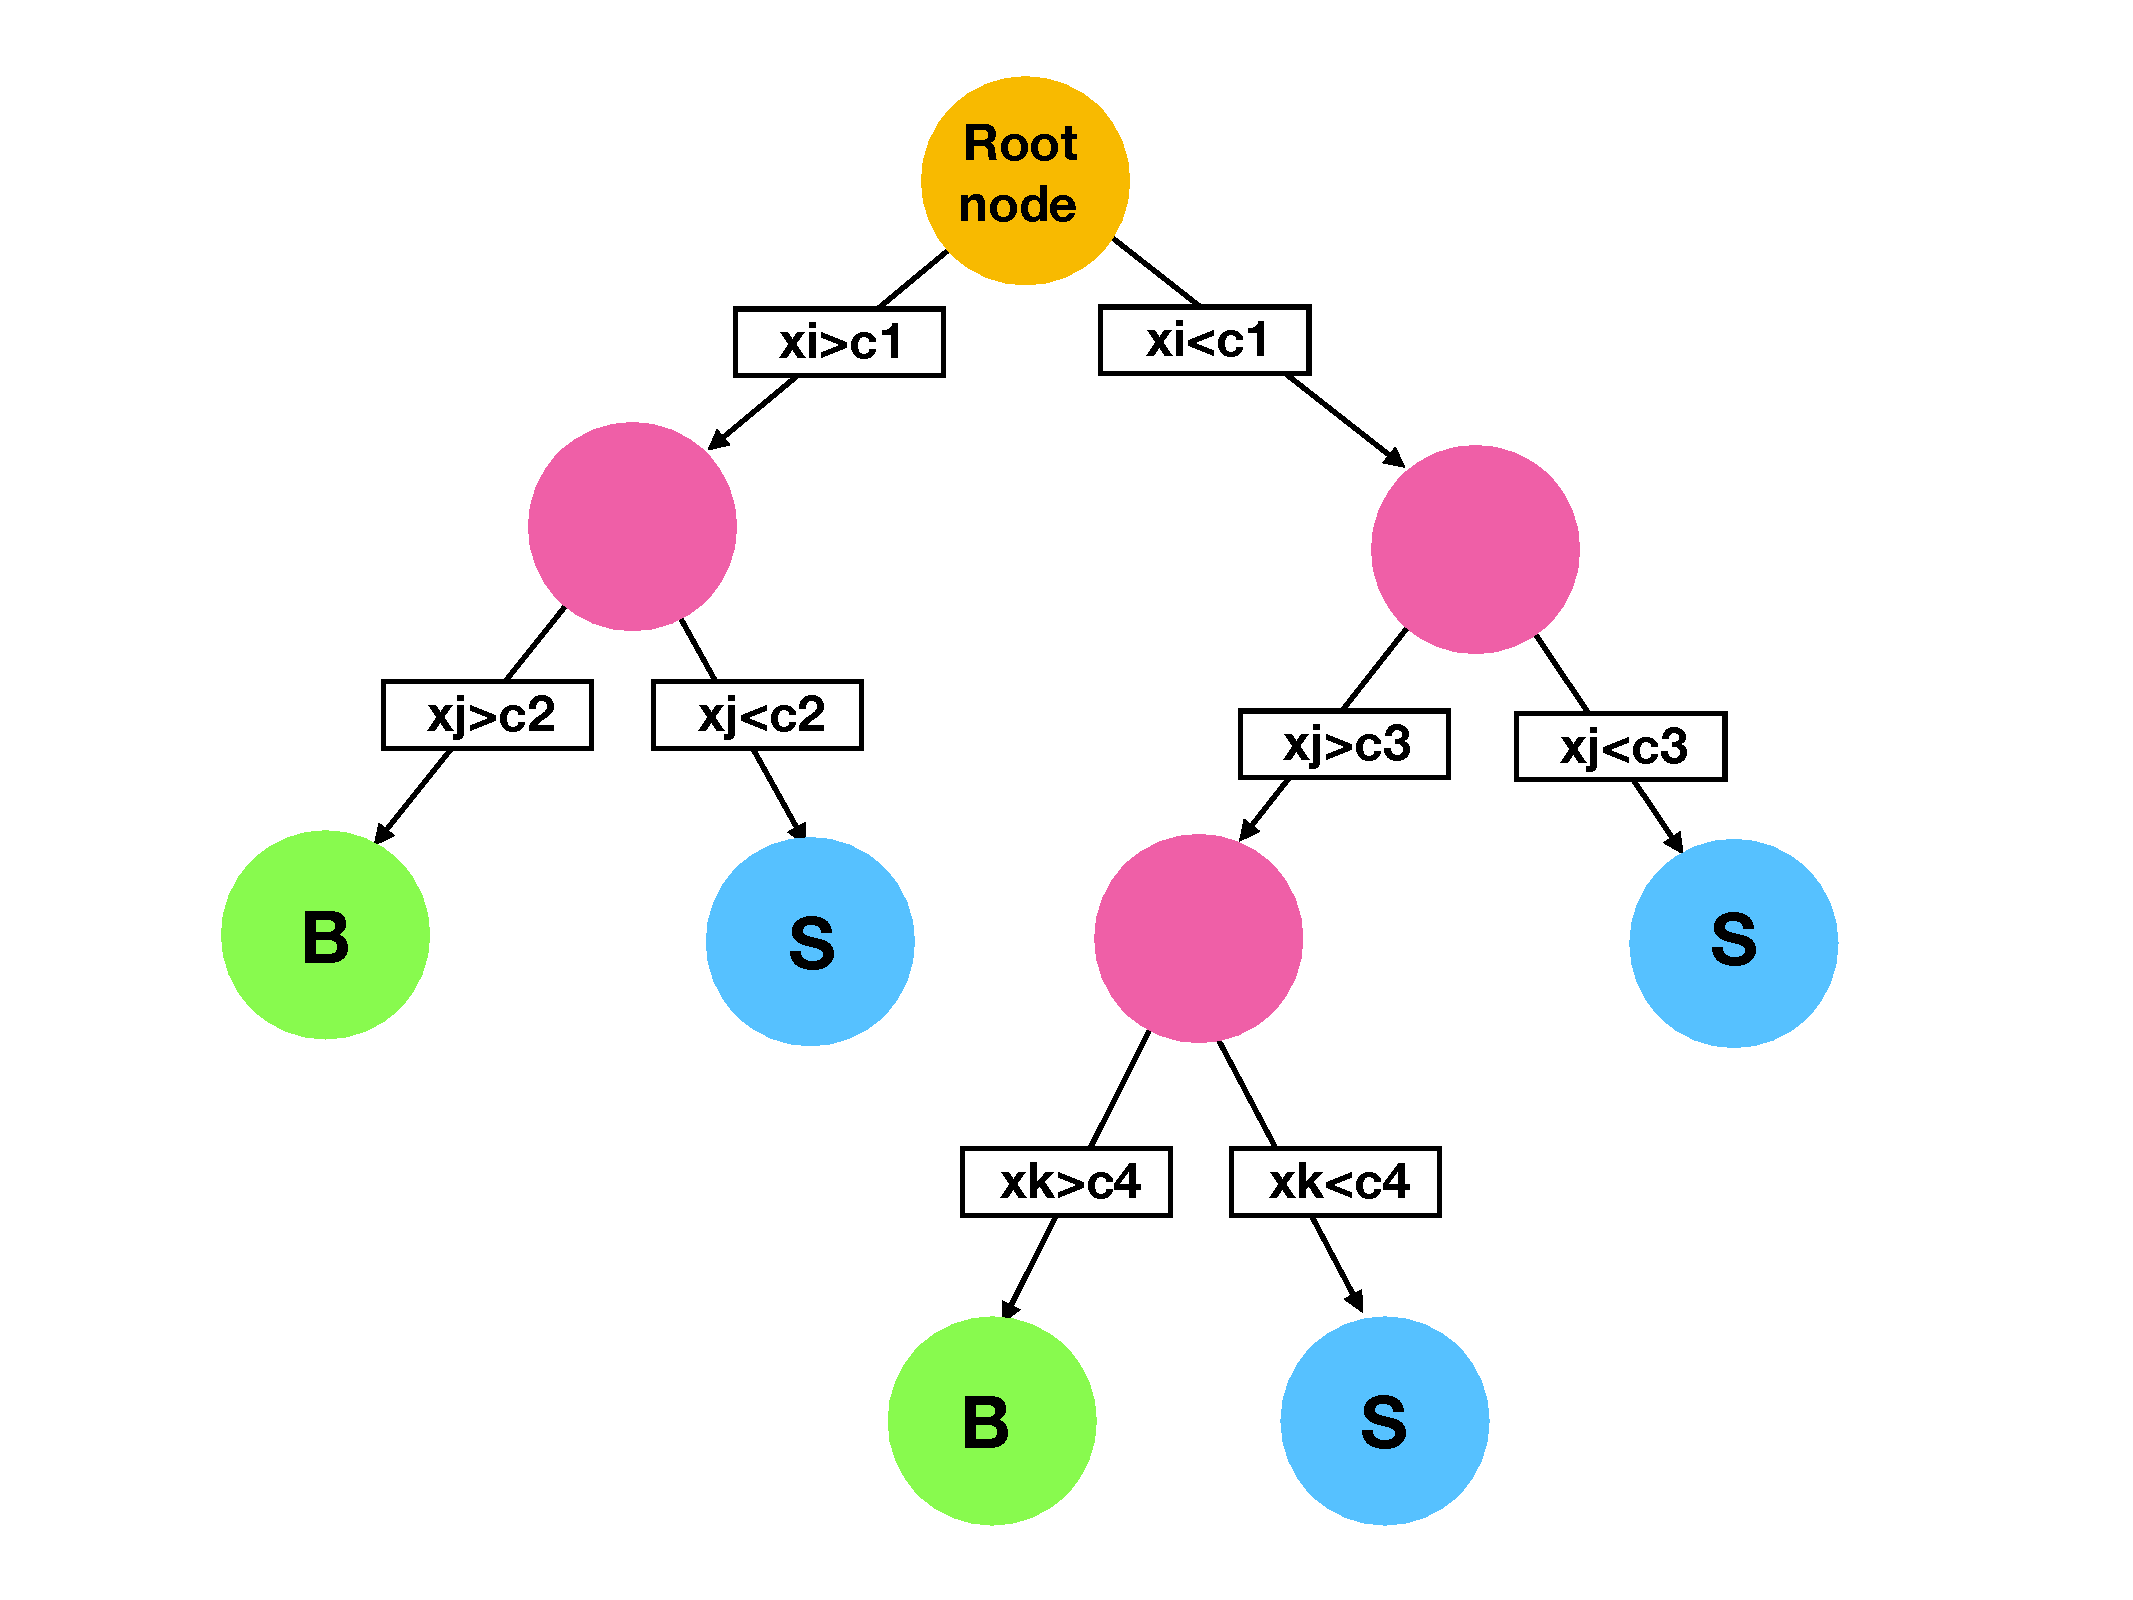
\includegraphics[width=0.6\textwidth]{chapter7/BDT_tree_show.pdf}
\caption{Tree structure example in BDT}
\label{fig:BDTtreestructure}
\end{figure}

Decision tree method is powerful, but the performance suffers from fluctuations. The selection of two variables with similar selection quality may be affected by a small change in the training sample. One of the solution is introducing the boosting algorithm. The boosting algorithm not only help stabilize decision tree training with respect to the small fluctuations inside the training data, but also enhance the classification.  AdaBoost is one of the boosting algorithms. With AdaBoost, after the first decision tree training, the misclassified events get higher even weights and as input into the second tree. Typically the AdaBoost training 1000 to 2000 trees. Misclassified event weights depend on the training error of each decision tree. Training error is calculated as in Equation.~\ref{Equ.errorBDT}, in which the superscript m, w are the tree label and event weight respectively. $y_{i}$ indicates the ith event type, 1 for signal and -1 for background. $T_{m}(x_{i})$ indicate the what kind of leaf event i with variable x lands on, 1 for signal leaf and -1 for background leaf. Variable $I(y_{i}\neq T_{m}(x_{i}))$ inside the Equation.~\ref{Equ.errorBDT} constructs on the variables $y_{i}$ and $T_{m}$ equal 1 if $y_{i}\neq T_{m}(x_{i})$ or 0 if $y_{i}= T_{m}(x_{i})$. As shown in Equation.~\ref{Equ.boostingweight}, with the intermediate quantity $\alpha_{m}$ for the tree m, the weight for event i is updated to its new value. While $\textrm{error}_{m}$ is required to be less than 0.5 so as the event weights are updated to the right direction. Learning rate parameter $\beta$ can be used to adjust the step of each re-weighting. The default value of $\beta$ is 1. Event weights in each tree is renormalized to keep the summed weights constant. The final score of each event after the boosting and training processes is obtained with Equation.~\ref{Equ.boostingeventweight}. High score indicates a signal like event while low score indicates a background ground like event.



\begin{align}\label{Equ.errorBDT} 
\textrm{error}_{m}=\frac{\sum_{i=1}^{N}w_{i}I(y_{i}\neq T_{m}(x_{i}))}{\sum_{i=1}^{N}w_{i}} 
\end{align}


\begin{align}\label{Equ.boostingweight} 
\alpha_{m}=&\beta\times \textrm{ln}((1-\textrm{error}_{m})/\textrm{error}_{m})\\
w_{i}\rightarrow &w_{i}\times e^{\alpha I(y_{i}\neq T_{m}(x_{i}))} \\
w_{i}\rightarrow &w_{i}/\sum_{i=1}^{N}w_{i}
\end{align}

\begin{align}\label{Equ.boostingeventweight} 
T(x)=\sum_{m=1}^{N_{tree}}\alpha_{m}T_{m}(x)
\end{align}



\section{Statistical methods}

The physics results are extracted with statistical methods. The limit of branching ratio with confident level(CL) method, significance and best fit branching fraction are mentioned in the analysis.  

Probability density function(PDF) and likelihood function are the base functions used. PDF of a continuous variable x can be interpreted as the likelihood of x at its different values. Probability density function holds the property that it is normalized to unity. 
\begin{align*}
\int f(x) dx =1
\end{align*}

Usually PDF of a variable interested accompanied with a set of parameters, so as PDF is usually written in the form $f(data|\alpha)$, which means the probability density function of variables in data  given the parameter set $\alpha$. These parameters can from various source, for example, from theory estimation, detector response and Monte Carlo simulation. All of the parameters in a model or a system, besides the parameters of interest, the other parameters that have an impact on the results are referred as nuisance parameters.       


Likelihood function of the same model $L(data|\alpha)$ is a function of parameter set $\alpha$ give data. In particle physics, Likelihood function more often in the form of $L(data|\mu,\theta)$, in which $\mu$ stands for signal strength modifier and $\theta$ stands for a full suite of nuisance parameters. Data in Likelihood function can be experimental data or pseudo-data which is produced to generate sample distribution. 
Taking the counting experiment as an example, PDFs and likelihood function in a binned sample can be estimated with poisson distribution as the PDF can be expressed as
\begin{align*}
f(data|u,\theta)=\prod_{i}\frac{(\mu s_{i}+b_{i})^{n_{i}}}{n_{i}!}e^{-\mu s_{i}-b_{i}}
\end{align*}
The $s_{i}$ and $b_{i}$ stand for the expected number signal and background events respectively and both of them are a function of nuisance parameter $\theta$ as $s_{i}(\theta)$ and $b_{i}(\theta)$. $n_{i}$ represents the number of events observed in bin i. The likelihood function in numerical form is similar to PDFs but implement the systematic error pdfs $\rho(\theta|\tilde{\theta})$ if there are systematics considered in the model~\cite{CMS-NOTE-2011-005}. The form of likelihood function can be expressed as 
\begin{align*}
\mathcal{L}=\prod_{i}\frac{(\mu s_{i}+b_{i})^{n_{i}}}{n_{i}!}e^{-\mu s_{i}-b_{i}}\cdot p(\tilde{\theta}|\theta)
\end{align*}

Both PDF and likelihood function rely on the knowledge of nuisance parameters. Auxiliary measurements or control regions are often used for the scale estimation of systematic uncertainties. With observations in different auxiliary measurements, a PDF $p(\tilde{\theta}|\theta)$ which is referred as the posteriors can be measured. Together with $\pi(\theta)$ which is referred as a prior, the systematic error pdfs can be constructed under the Bayes' theorem as
\begin{align*}
\rho(\theta|\tilde{\theta})\sim p(\tilde{\theta}|\theta)\cdot \pi_{\theta}(\theta)
\end{align*}
The systematic error pdfs can be improved and less affected by the choice of prior $\pi(\theta)$~\cite{statistics:school2016} by the auxiliary measurements. 

In the search of lepton flavour violaton higgs decay, the discovery will be finding the higgs events either decay into $\mu\tau$ pair in 13 TeV search or $e\tau$ pair in 8 TeV search.  LFV is forbidden in Standard Model(SM), thus, if take SM as a background only model, roughly speaking, a discovery can be claimed if the observation is not compatible with the background only model~\cite{LHCstaticstics}. To test the compatibility of the observed data with respect to the background only model and further calculate limits on the signal strength modifier of the signal+background hypothesis, the quantity test statistics and the PDFs of the two model under tested are needed.

Test statistics is a function which can map a set of data into a number. According to the Neyman-Pearson lemma, likelihood ratio of two model under test gives the most powerful test, which is expressed as
\begin{align*}
\tilde{q}_{\mu}=-2\textrm{ln}\frac{\mathcal{L}(data|\mu,\tilde{\theta}_{\mu})}{\mathcal{L}(data|\hat{\mu},\hat{\theta})}
\end{align*}
$\mu$ is the given signal strength modifier and $0<\hat{\mu}<\mu$. In the formula of $\tilde{q}_{\mu}$, $\tilde{\theta}$ is referred as conditional maximum likelihood estimator, given the signal strength modifier $\mu$, while in the denominator, $\hat{\mu}$ and $\hat{\theta}$ are allowed to flow freely to maximize the likelihood. The PDFs of signal+background model and background only model can be calculated in the following way. The observed $\theta^{obs}_{\mu}$ and  $\theta^{obs}_{0}$ for signal+background and background only model are obtained by maximizing the likelihood function respectively, also the observed $\tilde{q}_{\mu}^{obs}$ are calculated give $\mu$. The PDFs of signal+background model $f(\tilde{q}_{\mu}|\mu,\theta^{obs}_{\mu})$ and background only model $f(\tilde{q}_{\mu}|0,\theta^{obs}_{0})$ are constructed with the MC pseudo-data as shown in Figure.~\ref{fig:teststatistics}.

\begin{figure}[!tbp] 
\centering
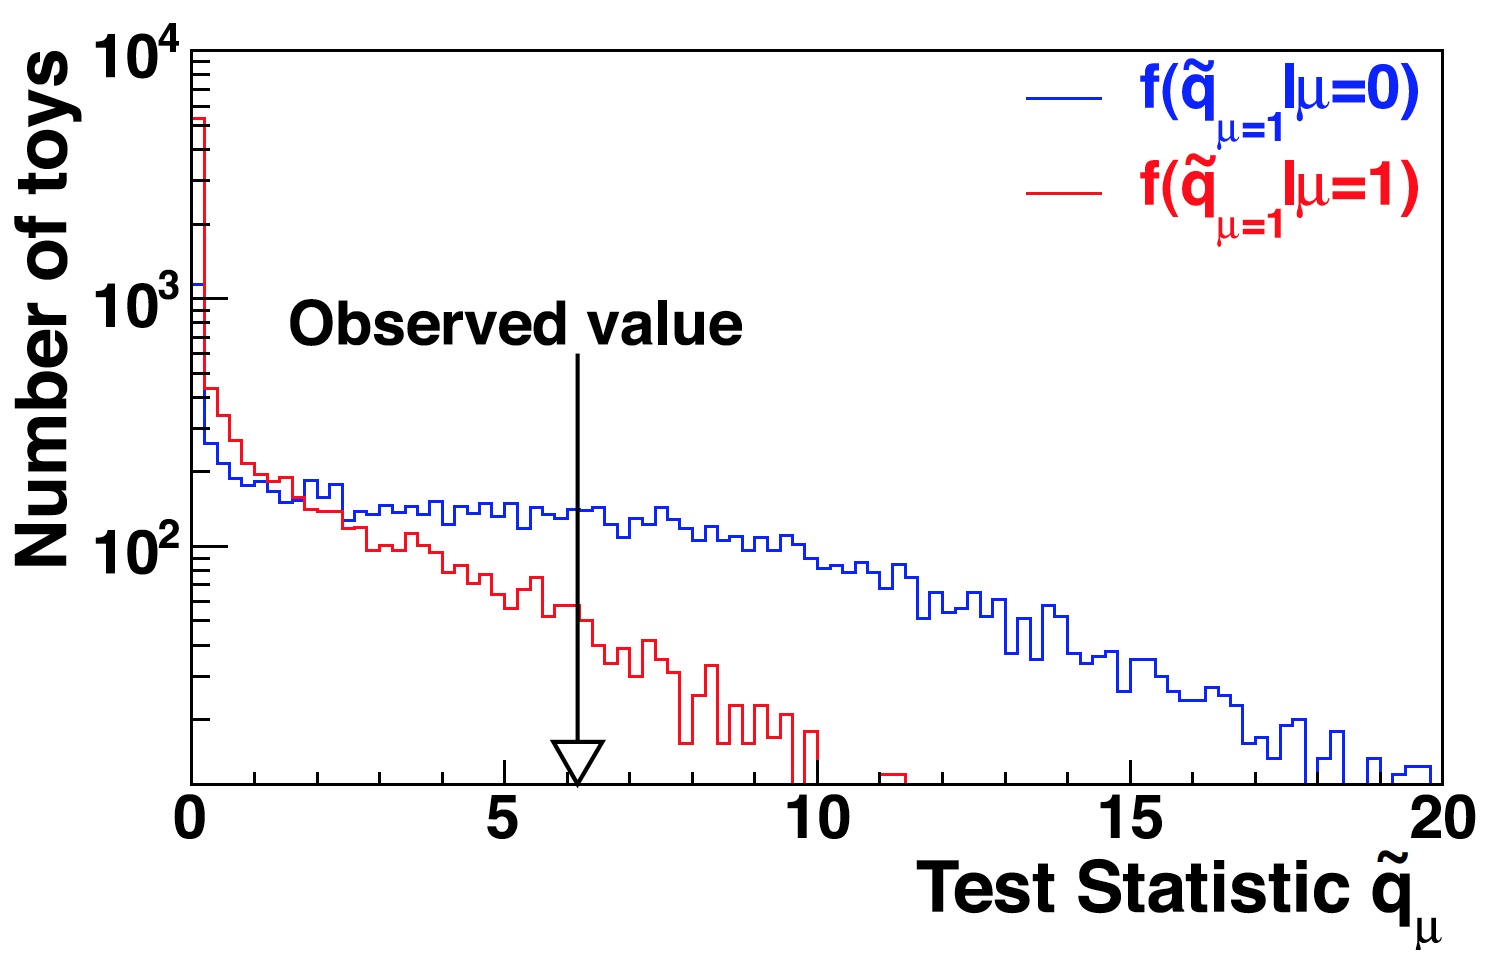
\includegraphics[width=0.6\textwidth]{chapter7/Test_statistics.png}
\caption{Test statistics distribution of signal+background and background only PDFs and the observed valued shown in arrow.}
\label{fig:teststatistics}
\end{figure}
 
Confident Level(CLs) are defined with two values $p_{\mu}$ and 1-$p_{b}$. In signal+background model, $p_{\mu}$ is defined as
\begin{align*}
p_{\mu}=P(\tilde{q}_{\mu}\geq  \tilde{q}_{\mu}^{obs}  |\textrm{signal+background})=\int^{\infty}_{\tilde{q}_{\mu}^{obs}}f(\tilde{q}_{\mu}|\mu,\hat{\theta}_{\mu}^{obs})d \tilde{q}_{\mu}
\end{align*}
In background only model 1-$p_{b}$ is defined as
\begin{align*}
1-p_{b}=P(\tilde{q}\geq  \tilde{q}_{\mu}^{obs} | \textrm{background only})=\int^{\infty}_{\tilde{q}_{0}^{obs}}f(\tilde{q}_{\mu}|0,\hat{\theta}_{0}^{obs})d \tilde{q}_{\mu}
\end{align*}

The $CL_{s}$ then is expressed as
\begin{align*}
CL_{s}=\frac{p_{\mu}}{1-p_{b}}
\end{align*}

With a given value of signal strength modifier $\mu$, $CL_{s}\leq\alpha$, then the signal+background is said excluded with $(1-\alpha)~ CL_{s}$. Usually $\alpha$ is picked as 95\%.

The expected limit shown in lepton flavour violation Higgs decay is the median 95\% $CL_{s}$ upper limit with the $\pm 1 \sigma$ and $\pm 2 \sigma$ bands in the background only model. By generating a large number of background only pseudo-data, the CLs and $\mu^{95\%}$ of each toy are calculated. An example of $\mu_{95\%}$ distributions is shown in Figure.~\ref{fig:Signal_strength_example}. As shown in the cumulative distribution of $\mu^{95\%}$, the median corresponds to 50\%,while $\pm 1 \sigma$, $\pm 2 \sigma$  correspond to range 16\% to 84\% and 2.5\% to 97.5\% respectively.     
\begin{figure}[!tbp] 
\centering
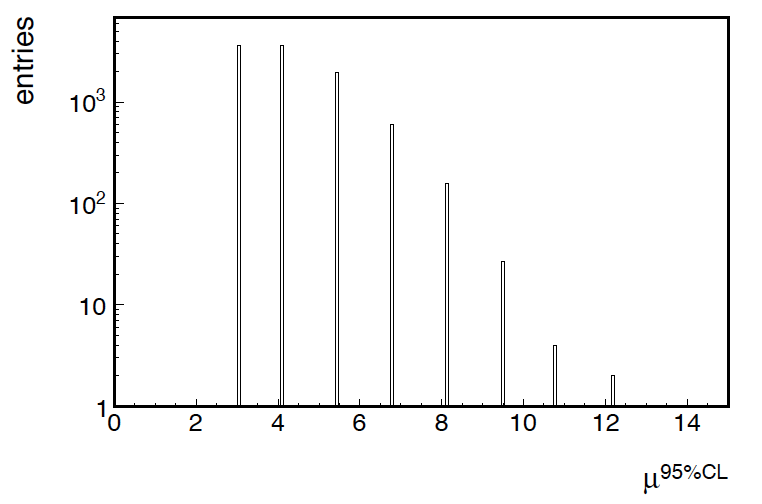
\includegraphics[width=0.4\textwidth]{chapter7/Signal_strength_example_1.png}
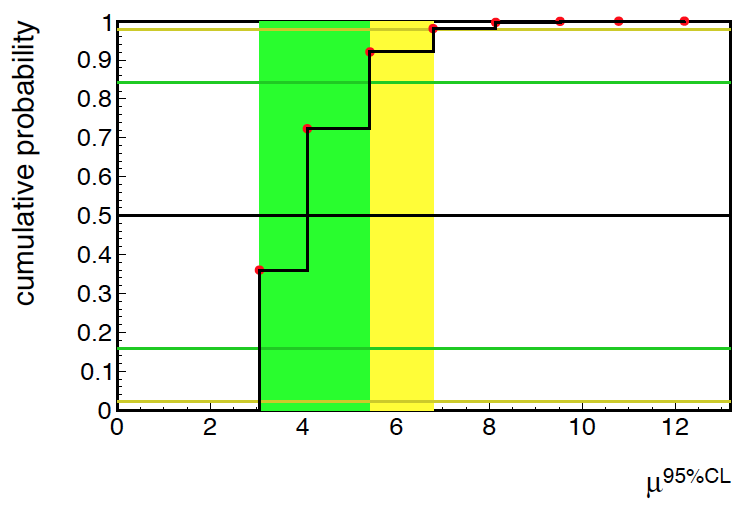
\includegraphics[width=0.4\textwidth]{chapter7/Signal_strength_example_2.png}
\caption{Signal strength modifier $\mu$ at 95\% $CL_{s}$ distribution from the MC pseudo-data. The right plot is the cumulative distribution of $\mu^{95\%}$ with $\pm 1 \sigma$ and $\pm 2 \sigma$ bands.}
\label{fig:Signal_strength_example}
\end{figure}

The estimator p value and significance are used to check if the data is compatible with background only model. Test statistics in the checking of background only model is expressed as
\begin{align*}
\tilde{q}_{\mu}=-2\textrm{ln}\frac{\mathcal{L}(data|0,\tilde{\theta}_{\mu})}{\mathcal{L}(data|\hat{\mu},\hat{\theta})}
\end{align*}
Similar procedure as mentioned above to get the PDF of background ground only model $f(q_{0}|0,\hat{\theta}^{obs}_{0})$ and $q^{obs}_{0}$. p-value corresponding to the experimental observable is calculated as

\begin{align*}
p_{0}=P(q_{0}\geq q_{0}^{obs})=\int^{\infty}_{q_{0}^{obs}}f(q_{0}|0,\hat{\theta}_{0}^{obs})d q_{0}
\end{align*}  
Significance Z of the observable with respect to the background only model test can be derived from p value~\cite{CMS-NOTE-2011-005}.
\begin{align*}
p=\int^{\infty}_{Z}\frac{1}{\sqrt{2\pi}}exp(-x^2/2)dx
\end{align*}  
The term used in the discovery as 5$\sigma$ correspond to Z=5 and p=$2.8\times10^{-7}$. The distribution of test statistics tends to  a chi-squared distribution as according to the Wilk's theorem, which gives a quick way of estimating of pdfs in test statistics~\cite{LHCstaticstics}. In the case when the expected number of events is large, expected limit with this asymptotic approximation gives a fairly well performance and save the computing time for toy samples. Asymptotic approximation can also used in the estimation of p value as
\begin{align*}
p^{estimate}=\frac{1}{2}\bigg[1-erf\bigg(\sqrt{q_{0}^{obs}/2}\bigg)\bigg]
\end{align*}  



\section{Systematics}
Systematic uncertainties originated from different sources that experimentally or theoretically affects the physics results. These uncertainties are considered by the effects on the normalization and shape of the distribution of different processes. 

\subsection{Systematics used in $\Hmuhad$}
The systematic uncertainties considered in this analysis are summarized in Table.~\ref{tab:systematicsone} and Table.~\ref{tab:systematicstwo}. The uncertainty on muon trigger, identification and isolation together amounts  to 2\% and the hadronic tau lepton efficiency amounts to 5\%. The uncertainties on lepton selections that include trigger, ID, isolation efficiencies are estimated Tag and probe method with Z boson data sets~\cite{Khachatryan2011,Chatrchyan:2012xi,Khachatryan:2015hwa,Khachatryan:2015dfa,CMS:2016gvn}. The systematic uncertainty of b tagging veto is taken from the uncertainty of b tagging veto efficiency measurement, which adjusts b tagging veto performance in simulation to match data samples. The exact values used in each category of $t\bar{t}$ and single top samples are in Table.~\ref{tab:btaguncertainty}. The uncertainties on $Z\to\tau\tau$, WW, WZ, ZZ, $t\bar{t}$, single top backgrounds mainly come from the uncertainties on the cross section measurement of each process. The normalization uncertainty of $\mu$ fake $\tau$ scale factor measurement and the uncertainty on $Z\to \mu\mu$ process together amounts to 25\%. An additional shape uncertainty of muon misidentifying tau is extracted from the measurement of the scale factor and treats independently of hadronic tau decay modes. $Z\to \mu\mu$ is the main source that contributes to $\mu$ fake $\tau$.  The uncertainty of the misidentified lepton background is estimated from the matching of the same sign control region which is defined as region II in Table.~\ref{tab:fakeratediagram}. The 30\% on normalization uncorrelated between each category and additional 10\% partially correlated within each category is a conservative estimation. Only the tau shape uncertainties are considered, which are taken from the variations of the misidentified tau parameters in fitting.  Muon misidentified shape uncertainty is omitted as it would be negligible compared with the bin-by-bin uncertainty applied.  The shape uncertainties of jet energy scale is estimated by varying the fitting parameters of different sources that affect this scale by one $\sigma$. Tau energy scale is treated as shape uncertainties and each of the tau decay modes is considered as independently. Unclustered energy refers to the energy loses from the jets $\pt<10$ GeV and the PF candidates that are not included in the jets reconstruction. The unclustered energy uncertainty is considered independently for charged particles, photons, neutral hadrons and very forward particles.  The uncertainties on Higgs boson cross section is affected by the renormalization scales, factorization, parton distribution functions(PDF) and the strong coupling constant($\alpha_{s}$). These affections in normalization are taken from \cite{YR4}.The uncertainties on Higgs cross section also affect the acceptance and result in the migration of events between categories.  The bin-by-bin uncertainty is applied to account for the statistics uncertainties within each bin. These uncertainties are uncorrected between different bins and categories. The uncertainty of integrated luminosity~\cite{CMS-PAS-LUM-17-001}  amounts to 2.5\%.



\begin{table}[htpb]
\caption{Part one of the systematic uncertainties considered in $\Hmuhad$ analysis. All of the uncertainties listed in the systematic tables are correlated between categories besides the ones after the sign $\oplus$. These are the uncertainties correlated in within each category but independent between categories. The theoretical uncertainties related to the acceptance and migration of events are listed in a range. The negative or positive values indicate a anticorrelated or correlated between categories}

%\caption{Part one of the systematic uncertainties considered in $\Hmuhad$ analysis. Systematic uncertainties in the expected event yields. All uncertainties are treated as correlated between the categories, except those that have two values separated by the $\oplus$ sign. In this case, the first value is the correlated uncertainty and the second value is the  uncorrelated uncertainty for each individual category. Theoretical uncertainties on VBF Higgs boson production~\cite{YR4}  are also applied to VH production. Uncertainties on acceptance lead to migration of events between the categories, and can be correlated or anticorrelated between categories. Ranges of uncertainties for the Higgs boson production indicate the variation in size, from negative (anticorrelated) to positive (correlated)}
\label{tab:systematicsone}
\centering
\begin{tabular}{l*{4}{c}} \hline
Systematic  uncertainty            & $\PH\to\Pgm\tauh$  \\ \hline
Muon  trigger/identification/isolation         &       2\%             \\
Hadronic tau lepton efficiency                  &       5\%              \\
b tagging veto                                          &      2.0--4.5\%     \\
$\PZ\to\Pgt\Pgt$ + jets background         &    10\%$\oplus$5\%   \\
$\PW\PW, \PZ\PZ$ background              &     5\%$\oplus$5\%       \\
\ttbar\  background                                  &     10\%$\oplus$5\%             \\
Single top quark background                 &     5\%$\oplus$5\%  \\
$\Pgm\to\tauh$ background                                      &         25\%         \\
$\text{Jet}\to\tauh, \Pgm $ background             &  30\%$\oplus$10\%   \\
Jet energy scale                                                       &   3--20\% \\
\tauh energy scale                                                    &   1.2\%  \\\hline
\end{tabular}
\end{table}



\begin{table}[htpb]
\caption{Part two of the systematic uncertainties considered in $\Hmuhad$ analysis}
\label{tab:systematicstwo}
\centering
\begin{tabular}{l*{4}{c}} \hline
Systematic  uncertainty                                             & $\PH\to\Pgm\tauh$ \\ \hline

$\Pgm \to\tauh$ energy scale                                   &    1.5\%  \\
\Pgm\ energy scale                                                   &        0.2\%      \\
Unclustered energy scale                                         &        $\pm 1 \sigma$  \\
Renorm./fact. scales ({\Pg\Pg}H)   \cite{YR4}          &   \multicolumn{4}{c}{3.9\%}\\
Renorm./fact. scales (VBF and VH) \cite{YR4}         &   \multicolumn{4}{c}{0.4\%}\\
PDF + $\alpha_s$ ({\Pg\Pg}H)    \cite{YR4}             &   \multicolumn{4}{c}{ 3.2\%}\\
PDF + $\alpha_s$ (VBF and VH)   \cite{YR4}          &   \multicolumn{4}{c}{ 2.1\%}\\
Renorm./fact. acceptance ({\Pg\Pg}H)                     &   \multicolumn{4}{c}{$-3.0$\% -- $+2.0$\% } \\
Renorm./fact. acceptance (VBF and VH)                &   \multicolumn{4}{c}{$-0.3$\% -- $+1.0$\% } \\
PDF + $\alpha_s$ acceptance ({\Pg\Pg}H)              &   \multicolumn{4}{c}{ $-1.5$\% --  $+0.5$\%}\\
PDF + $\alpha_s$ acceptance (VBF and VH)          &   \multicolumn{4}{c}{ $-1.5$\% --  $+1.0$\%}\\
Integrated luminosity               &   \multicolumn{4}{c}{ 2.5\%  } \\ \hline
\end{tabular}
\end{table}

\begin{table}[htpb]
\caption{b tagging veto systematic uncertainty in each category}
\label{tab:btaguncertainty}
\centering
\begin{tabular}{lclclclcl}\hline
                       & 0 jet    &  1 jet       & 2 jets gg-enriched & 2 jets VBF-enriched \\\hline
$t\bar{t}$        &  \NA    &  2.45\%    &4.37\%                   & 2.59\%     \\   
$t$   & \NA     &  2.11\%    & 3.07\%                   & 1.98\%   \\\hline
\end{tabular}
\end{table}







\subsection{Systematic uncertainties in $\Hehad$}

The systematic uncertainties affect the $\Hehad$ analysis are summarized in Table.~\ref{tab:systematics_had}, \ref{tab:theory_systematics} and \ref{tab:shape_systematics}, which includes the ones affect the normalization and the ones affects the shape of $\mcol$ distribution. The uncertainty of the electron measurements, which include the trigger, ID and isolation come from the Tag and Probe measurement with Z boson datasets \cite{CMS:2011aa,Khachatryan:2015dfa}. The uncertainties from the $\PZ \to \tau \tau$ is from the uncertainty of the cross section measurement~\cite{Chatrchyan:2014mua} and the $\tau$ identification in the embedded technique. The normalization uncertainty on $\PZ \to \Pgm \Pgm$ amounts to 30\% which is the from the measurement of cross section and statistics uncertainty in the yields. An extra 5\% shape uncertainty due to the mismeasured energy of the electron reconstructed as $\Pgt$ in $\PZ \to \Pe\Pe$ background.  The shift in $\mcol$ distribution is measured by comparison between data and MC simulation. The uncertainty in misidentified tau lepton background is 30\% normalization uncertainty correlated between categories and shape uncertainties. The shape uncertainties is obtained by varying the parameters from fitting the fake ratio one standard deviation.   The uncertainty from the pileup process are estimated by varying the total inelastic cross section by $\pm5$ percentage~\cite{Chatrchyan:2012nj}. The uncertainty from Diboson, single top quark background is taken from the measurement of the cross section. In $t\bar{t}$ background, the uncertainty in 0 jet, 1 jet category are taken from the cross section measurement, in 2  jets category, an extra 33\% uncertainty uncorrelated between categories is added due to the statistical uncertainty. The luminosity uncertainty amounts to 2.6\%.  Jet energy scale(JES) and resolution is measured with $\gamma/\PZ+jets$ and dijet data~\cite{CMS-JME-10-011}. The uncertainty from JES is applied as a function of $\pt$ and $\eta$. Jet energy resolution(JER) uncertainty is obtained by smearing jets energy as a function of $\pt$ and $\eta$. Both JES and JER affect the shape of $\mcol$ distribution and are taken as shape uncertainties. The energy of the jets below 10 GeV and PF objets that are not clustered are accounted as the unclustered energy scale, which is also taken as shape uncertainties. The uncertainty of $\tau_{h}$ energy scale is from the comparing $\PZ \to \tau\tau$ distruction between data and MC sample and applied as a shape uncertainty. The theoretical uncertainties considered in the $\Hehad$ analysis are listed in Table.~\ref{tab:theory_systematics}. There are several sources that contribute to the theoretical uncertainties and considered fully correlated between LFV Higgs and SM Higgs production. The uncertainty in Parton distribution function is obtained by counting the yields with different PDFs,  CT10~\cite{Nadolsky:2008zw}, MSTW~\cite{Martin:2009iq}, NNPDF~\cite{Ball:2010de}  from the recommendation in PDF4LHC~\cite{Botje:2011sn}. The uncertainty in renormalization and factorization scales are from scaling up and down by a factor of two to their normal values($\mu_{R}=\mu_{F}=M_{H}/2$). The uncertainty in underlying events and parton shower is estimated by checking with different PYTHIA tunes. The theoretical uncertainties are all correlated or anticorrelated which have a minus superscript and are the results of the events migration.   




\begin{table*}[hbt]
 \centering
 \caption{The normalization systematic uncertainties considered in $\Hehad$ analysis. The uncertainties are correlated between categories besides the ones after $\oplus$. These uncertainies are uncorrelated between categories. }
  \label{tab:systematics_had}
\begin{tabular}{l|c|c|c} \hline
Systematic uncertainty                  & \multicolumn{3}{c}{\PH$\to \Pe\tauh$}      \\ 
                                                      & 0-jet       & 1-jet        & 2-jet                 \\ \hline
Electron trigger/ID/isolation           &  1\%           &   1\%         &  2\%                       \\
Efficiency of $\tauh$                      &  6.7\%         &  6.7\%        & 6.7\%                      \\
$\PZ\to \Pgt \Pgt$ background    & 3\%$\oplus$5\% & 3\%$\oplus$5\%& 3\%$\oplus$10\%            \\
$\PZ\to \Pe\Pe$ background                      & 30\%           &  30\%         & 30\%                       \\

Misidentified leptons background                   & 30\%           &  30\%         & 30\%                       \\
Pileup                                           & 4\%           & 4\%          & 2\%                       \\
$\PW\PW,\PW\PZ,\PZ\PZ\mathrm{+jets}$ background                 & 15\%           &  15\%         & 15\%                       \\
$\ttbar$ background                     & 10\%           &  10\%         & 10\%$\oplus$33\%           \\
Single top quark background       & 25\%           &  25\%         & 25\%                      \\
Luminosity                                    & 2.6\%          &  2.6\%        & 2.6\%                      \\ \hline
\end{tabular}
\end{table*}


\begin{table}[hbtp]
 \centering
 \caption{The systematic uncertainties that affect the shape of $\mcol$ distribution. }
  %\caption{Systematic uncertainties in the shape of the signal and background distributions, expressed in percentage. The systematic uncertainty and its implementation are described in the text.}
  \label{tab:shape_systematics}
  \begin{tabular}{lclc} \hline
Systematic Uncertainty                                 &   $\PH \to \Pe \tauh$                   \\ \hline
$Z \to \Pe\Pe$ bias                                       &   5\%                                         \\
Jet energy scale                                           &    3\%--7\%                                       \\
Jet energy resolution                                    &    1\%--10\%                                       \\
Unclustered energy scale                             &    10\%                                       \\
$\tauh$ energy scale                                    &    3\%                                         \\    \hline
  \end{tabular}
\end{table}



\begin{table*}[hbtp]
 \centering
 \caption{Theoretical uncertainties that affects the Higgs boson production cross section. These uncertainties are correlated or anticorrelated(with minus sign superscript) between all of the categories.}
 % \caption{Theoretical uncertainties in percentage for the Higgs boson production cross section for each production process and category. All uncertainties are treated as fully correlated between categories except those denoted by a negative superscript which are fully anticorrelated due to the migration of events.}
  \label{tab:theory_systematics}
  \begin{tabular}{l|l|l|l|l|l|l} \hline
Systematic uncertainty                  &  \multicolumn{3}{c|}{Gluon fusion} &  \multicolumn{3}{c}{Vector boson fusion}  \\ \cline{2-7}
                                &    0-jet  & 1-jet  & 2-jet   & 0-jet & 1-jet  & 2-jet  \\ \hline
Parton distribution function         &    $9.7$\%  &  $9.7$\% &   $9.7$\% & $3.6$\%  &   $3.6$\%  &  $3.6$\%  \\
Renormalization/factorization scale           &    $8$\%    &  $10$\%   &  $30^{-}$\%   & $4$\%     &   $1.5$\%  & $2$\%   \\
Underlying event/parton shower  &   $4$\%     & $5^{-}$\%   &  $10^{-}$\%   & $10$\%    &   $<$1\%    & $1^{-}$\%   \\ \hline
  \end{tabular}
\end{table*}


       




